\subsection{Benchmarks}
\label{subsec:benchmark}

\paragraph{Frequency of Updates}
To determine the frequency of updates, values received per second where averaged over 100 seconds.
The rate of updates from the gyroscope is very steady, at between 31 and 32 Updates per second.
The frequency of new values from the ultrasound sensor is not as steady, as it depends on the distance being measured.
This is because longer distances take longer to measure, and the arduino immediately starts a new measurement upon completion.
In general, distance measured and update frequency are inversely proportional, i.e. with longer distance the rate of updates decreases.
At 10cm distance, update frequency is about 75Hz, and decreases roughly by about 10hz per meter, see \ref{fig:benchmark}.

\begin{table}
    \centering
    \begin{tabular}{l|lll}
            & Gyroscope & Ultrasound & \\
        \cline{1-3}
        10  & 31.48979  & 74.9898    & \\
        20  & 31.48979  & 73.77319   & \\
        30  & 31.55670  & 72.02040   & \\
        50  & 31.57731  & 73.82653   & \\
        75  & 31.62886  & 72.11224   & \\
        100 & 31.60821  & 65.42857   & \\
        150 & 31.50515  & 55.66326   & \\
        200 & 31.62244  & 53.83673   &
    \end{tabular}

    \caption{Distance in cm from sensor and update frequency}
    \label{table:benchmark}
\end{table}

\begin{figure}
    \centering
    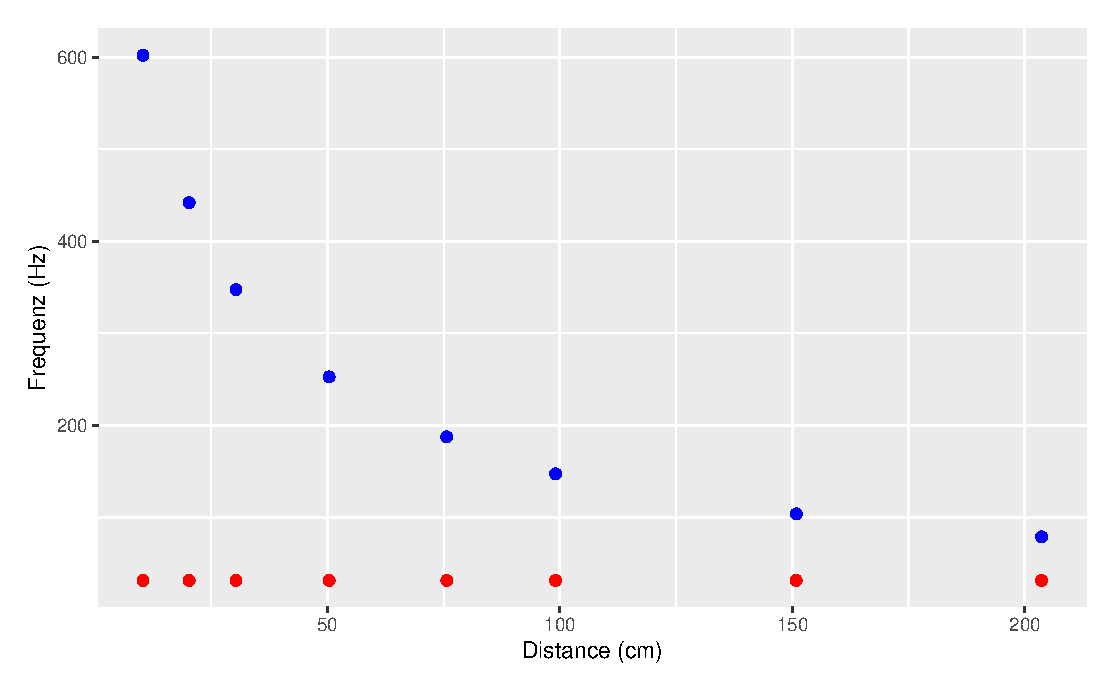
\includegraphics[width=0.5\linewidth]{figures/benchmark.eps}
    \caption{The data from \ref{table:benchmark} visualized}
    \label{fig:benchmark}
\end{figure}

